\chapter{Improved Melanoma Detection using Asymmetry}

\section{Introduction}

Melanoma is a type of malignant skin cancer that accounts for a significant proportion of cancer-related deaths around the world. In 2018 there were approximately 2,353 per 100,000 deaths in the United Kingdom (UK)\cite{UK2019}. Early detection is critical for improving the diagnosis and survival of patients. However, existing approaches including clinical examinations and dermoscopy, have limitations in terms of accuracy and cost-effectiveness\cite{Takiddin2021}. Machine learning approaches have beaten dermatologists in terms of accuracy\cite{Andre2017}. However, these approaches lack explainability implementing such techniques difficult for clinical environments\cite{Fan2017}. One concern is the production of realistic, but incorrect results\cite{Ghorbani2019}. Another is the use of parallel processes, which describes the creation of an answer with little to no explanation. In this paper, we propose a combined asymmetry approach using shape, colour, and texture analysis alongside a detailed comparison. The technique itself can be used in conjunction with ABCD rules (Asymmetry, border, colour, dermoscopic features).

\section{Related Works}
% Quick summary of TDS, ABCD rules, bi-fold and general issues
Asymmetry analysis is a fundamental component in the early detection of melanoma because it often exhibits asymmetric shapes\cite{Ali2020a}. Meaning that the shape, colour and, texture matches asymmetrically more often in benign lesions. Bi-fold is a diagnostic procedure designed to recognize melanoma by drawing a line down the middle of the skin lesion and comparing the two halves to confirm whether the sides match (considering the difference in shape, colour, and texture). Using this horizontally and vertically calculates whether the skin lesion is possibly malignant with a score between 0 and 2. Calculating with Total Dermoscopy Score (TDS) alongside the other ABCD rules including asymmetry, border, colour, and diameter calculates the likelihood of malignancy. Dermatologists frequently use bi-fold due to its simplicity, but it can be subjective to the original observer and time-consuming when managing large numbers of skin lesions. Therefore, automating techniques is beneficial to clinicians and can improve the objectivity of results.

% Measuring asymmetry shape
Ihab S. Zaqout\cite{Zaqout2016} describes a technique using the centroid and rotation of the skin lesion using moments of inertia. By Folding the skin lesion on both vertical and horizontal axes subtracting the opposite half. Pixels that cannot subtract are summed and compared with a threshold considering the skin lesion asymmetrical if the combined sum is more than the threshold.

% Measuring asymmetry colour
Kasmi and Mokrani\cite{Kasmi2016} create a grid of 20 by 20 pixels from the skin lesion image and convert it into the LAB colour space. They then compare the average colour of each block with a perpendicular block (vertical and horizontal axes) using the three-dimensional Euclidean luminance distance, a-axis, and b-axis. If more than half of the colour comparisons exceed the threshold, they consider that axis to be colour asymmetrical. They ignore blocks that have no symmetrical pair. Finally, they calculate luminance separately to prevent brightness problems. This technique achieves an accuracy of 94\% with a private dataset.

% Measuring asymmetry texture
Ali\cite{Ali2020a} uses SIFT-based similarity and projection profiles to measure similarities in texture. SIFT is scale-invariant and helpful for texture components with varying texture quality. First, they split the skin lesion vertically and horizontally across the centre into four halves, compare texture components on the symmetrical halves, and measure similarity. Lastly, they generate histograms for the projection profile in the x and y directions. These results train a decision tree and achieve an 80\% accuracy of the ISIC 2018 with 204 images privately annotated for ABCD rules.

% Summary of techniques and mention of the proposed approach
Prior studies have introduced techniques that measure distinct aspects of asymmetry, such as Ihab S. Zaqout\cite{Zaqout2016} measurement of shape, Kasmi and Mokrani\cite{Kasmi2016} measurement of colour, and  Ali\cite{Ali2020a} measurement of texture. The new approach seeks to combine the following approaches into a more comprehensive analysis of asymmetry that takes into account multiple features of the skin lesion. The proposed novel technique updates colour measurement to improve accuracy using superpixels and an SVM model.

\section{Novel Asymmetry Analysis Approach}
To initiate the classification of skin lesions a technique called bi-fold is applied involving folding the skin lesion in half vertically and horizontally and a comparison of their respective dimensions. While the original technique was designed only to assess the lesions' shape, it's been utilized to account for colour and texture as well. The centre and orientation are determined by calculating its moments, where the centre is (m10 / m00, m01 / m00) and phi is 0.5tan (2m11)/ (m20 -m02). 

Next, the lesion is partitioned into a 20 by 20 grid centred on the mentioned centre point, and the average of each region is computed. This is followed by finding the matching region on the perpendicular area from the centre of the skin lesion and comparing the colour distance between the two. Distance is measured using the LAB colour space and a 2d Euclidean distance of A and B, removing L (luminosity) to eliminate light variation. Once compared, all compared regions are obtained, and they are plotted onto a graph. If over half of the values are above a threshold of 6, then the lesion is asymmetrical.

% Scrutinize the threshold method and show the graph that the data can't be split with only the threshold 
The diagram shown below in \ref{symmetrical} is a compilation of all the images within the PH\^2 dataset showing the threshold range after applying bi-fold, euclidean distance of colour, but before applying the threshold. As can be seen a threshold of 6 covers all of the symmetrical values, but still roughtly covers half of the asymmetrical values. This demonstrates that the technique produces many false positives when regarding asymmetrical values.
Essentially, the symmetrical skin lesion has a smaller area and the asymmetrical lesion has a larger area, but both remain in the same zone and therefore splitting the data only using a threshold holds poor results. Furthermore, there are a lot of fliers and the threshold does not adjust according to these values. See the graph below:

\begin{figure} 
    \centering
    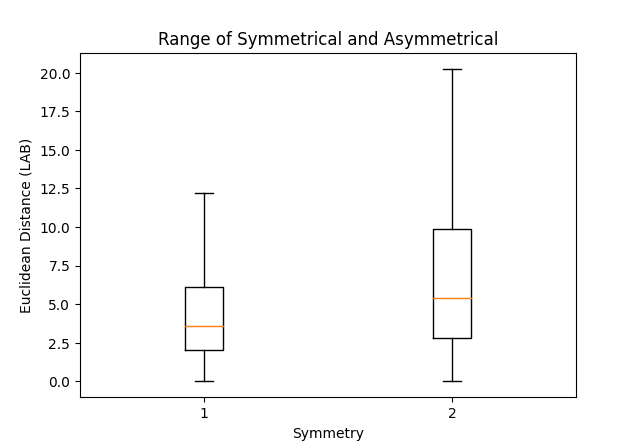
\includegraphics[scale=0.6]{images/symmetrical.png}
\caption{This diagram is a summary of the PH2 dataset after using bi-fold, euclidean distance of colour. The value on the right would be a threshold.}
\end{figure} \label{symmetrical}
    
To improve the accuracy of the algorithm some changes need to be made based on the previous statements. First will be superpixels and next is k-means.

% Demonstrating the changes including superpixels and graphs, etc
Superpixels is an algorithm for grouping pixels into a region with similar values. This one uses simple linear iterative clustering (SLIC) algorithm\cite{Achanta2012} to do so. The goal of using this instead of averaging specific areas as shown in\cite{Kasmi2016}, is to segment areas of similar interest values. This is to prevent areas from being cut in half.

The image in ... demonstrates the usual average and the new averages based on superpixels and the changes in values. Areas that are lighter in colour appear to have a lower value and darker appear darker.

Using the thresholding method for classification we can already see the accuracy has been improved with a threshold of ...

\section{Results}
The goal of this experiment is to improve the accuracy of the asymmetry bi-fold technique described by Ihab S. Zaqout et al.\cite{Zaqout2016}. Initially, the skin lesion is split into a 10 by 10 grid and converted into the LAB colourspace. Next, a line is drawn through the middle horizontally and vertically. Measuring the euclidean distance from the centroid, locating the closest opposite patch of colour finds the parallel square. Subtracting the squares generates a score for each value, the closer to 0, the more similar the colour. These are then removed from the list to prevent them from being selected a second time. If half the results are over a specific threshold, it is considered asymmetrical in colour, otherwise considered symmetrical. The aim is to make a 10 by 10 grid, but instead of averaging squares, superpixels reduce data redundancy in the grid, allowing for a less complex algorithm and improving accuracy. The clustering method k-means partition each pixel to its nearest most similar centroid relating to colour. Next, it generates a superpixel that represents the average colour of that area. The diagram \ref{SP} demonstrates different borders when changing the $C$ for compactness, where 100 generates a square grid similar to the original technique. The border becomes more flexible as the compactness value decreases.

\begin{figure} 
\centering
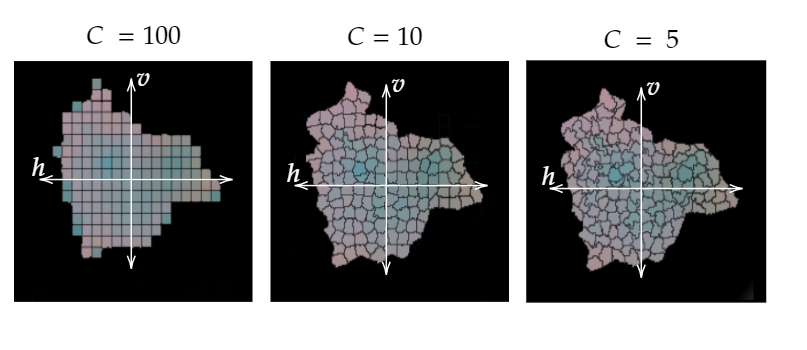
\includegraphics[scale=0.6]{images/superpixels.png}
\caption{This diagram shows the skin lesion split relating to superpixels instead of averaging squares.}
\end{figure} \label{SP}

Each parallel square on the vertical and horizontal axes measures similarity using a three-dimensional euclidean distance in the LAB colour space. For example, the perceivable difference of colour to the human eye is a three-dimensional euclidean distance of 6\cite{Myridis2014a}. Using similar logic, a value of 20 is the threshold, where any value over that amount is considered asymmetrical in colour. Next, each square is compared with its closest parallel square and removed from an array after being compared. The next improvement is to generate a unique threshold for the significance of each square. For example, using superpixels with the compactness of 10 has an accuracy of 61\% with the PH$^2$ dataset compared to the original 59.5\%. This approach demonstrates that a flexible border that considers features is more effective than averaging squares.

\begin{figure}
\centering
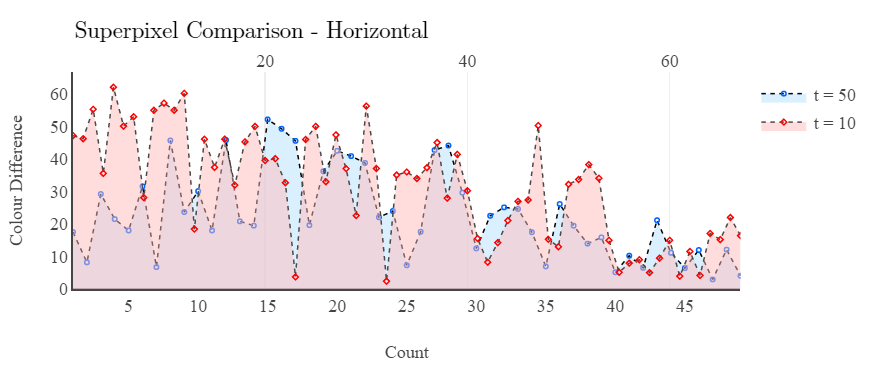
\includegraphics[scale=0.7]{images/superpixel2.png}
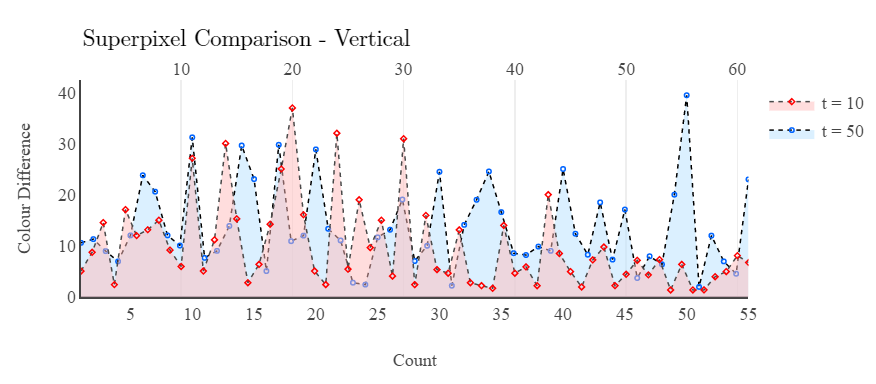
\includegraphics[scale=0.7]{images/superpixel1.png}
\caption{This diagram shows the difference between averaging squares and using superpixels, with the threshold of 10 implying curves and 50 being square. The horizontal colour difference is improved, making it more likely to be seen asymmetrical. The vertical comparison is roughly the same, except for removing a false positive of 40.}
\end{figure} \label{asy3}

There is a correlation in colour differences between the inner and outer edges because melanoma typically expands outwards, creating an abnormal border. This information specifies that the statistical model accuracy could be improved by increasing the threshold for the outer edges and decreasing for the inner.


\subsection{Removing}

% Describe the asymmetry technique and the changes that have been made to it.
The proposed method has many similarities to Kasmi and Mokrani\cite{Kasmi2016} colour comparison technique, except it is updated to improve accuracy using superpixels, and a Support Vector Machine (SVM).

The original method uses moments of inertia

without any flexibility splits areas of interest in half, making comparisons less adequate. Using superpixels allows for a softer border which improves colour separation and accuracy.

Superpixels are k-means colour extraction techniques designed to separate areas of an image into their associated areas of colour by applying a soft border around the edge. 